\section{Resource Utilization}

It is possible to configure resource utilization in Kubernetes through configuration options called \textit{limits} and \textit{requests}. Requests dictates the resources that a running pod \textbf{must} have and limits set up resources that a running pod \textbf{can} have at maximum utilization. Requests and limits protect pods from starving for resources and provides an artificial performance isolation. Figure \ref{fig:limits} shows how Kubernetes operates with those constraints.
\begin{figure}
    \centering
    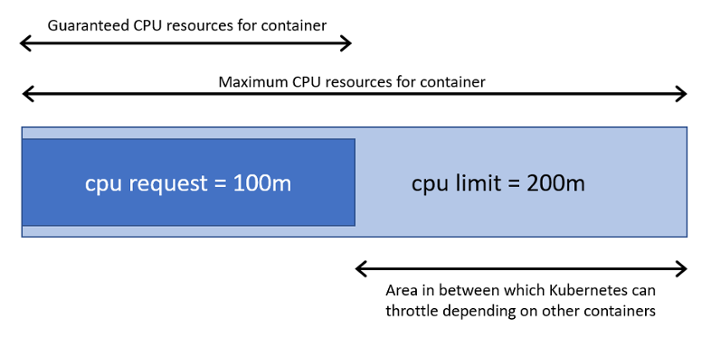
\includegraphics[width=0.9\textwidth]{container-resource-1.png}
    \caption{Kubernetes resource utilization \cite{limits}}\label{fig:limits}
\end{figure}

Similar configuration also exists in Xen hypervisor. \textit{mem-max} argument to the command line interface \textit{"specifies the maximum amount of memory the domain is able to use"} \cite{xl-man-page}. This option will be passed as a limit in the pod deployment template and will be parsed by the virtual-kubelet to use in the command. \textit{vcpu-pin} command \textit{"sets hard and soft affinity for a vcpu of <domain-id>}". Similar to memory option, this option can also be passed in the template file. Xen also has additional configuration for its own scheduler that aligns well with Kubernetes. For example, \textit{weight} flag assigns a priority to a VM and that priority is used when requesting resources. It can be seen in figure \ref{fig:xenoutput}. \textit{Cap} flag \textit{"fixes the maximum amount of CPU a domain will be able to consume"}. This command operates on CPUs and not on VCPUs.

When booted by the Xen hypervisor, unikernels act similar to virtual machines and they have the same performance isolation problems as VMs. Chi et al. \cite{performance-isolation} find that Xen has performance isolation problems and they argue that VMEXIT behavior is the most important reason for that. In Kubernetes, by design, many pods are ephemeral and this means many VMEXIT behavior will be observed when running pods with Xen. This might create performance isolation problems for big deployments.

Deschane et al. \cite{Deshane} argue that Xen shows poor isolation performance for network sender and network receiver operations. Kubernetes is a highly connected system, and many deployed unikernel will have a network component. This might also hinder better performance isolation. They also argue that KVM is better on isolating network sender but not on network receiver operation. They state Xen scales better than KVM, which makes it a better candidate for high replica scenarios.